% !TEX root = ../seapp-manual.tex

% Appendix C - Create and fill packets properly

\chapter{Create and fill packets}
\label{ch:appendix-C}

This chapter shows informations that may help the user to create and fill a packet properly. To build a packet from scratch that belongs to a certain layer, the user has to know its structure and the protocol that runs on the layer below or above. The user has also to know the output gate of the local filter (or local filters) to which forward the packet.

\section{Create new packet}

To create a new packet, the user has to define the ADL type of the packet in the \emph{create} action. The table \ref{tab:from5-to4} presents the assigned ADL types to the existing application packets and the control info objects which are attached to them.

In case of a new type of packet which is not supported by SEA++, the user has to extend the implementation of SEA++ by adding the new type. To do so, the \emph{Create.h}, \emph{Create.cc} and the \emph{seapputils.cc} files has to be modified. More in details:
%
\begin{itemize}
\item Create a new application packet (\emph{.msg})
\item Extend the \emph{type\_t} enum class in the \emph{/actions/create/Create.h} file by writing the name of the new packet;
\item Extend the \emph{buildNewPacket(cPacket** packet, int layer, type\_t type)} method of \emph{/actions/create/Create.cc} file to create a new application packet;
\item Extend the \emph{getPacketLayer(cPacket* packet)} method of \emph{/util/seapputils/seapputils.cc} to return the layer of the new packet.
\end{itemize}

\section{Handle ControlInfo object}

After the creation of a packet, the user has to fill its header by using the action change. In some cases the user has also to fill the fields contained in the \texttt{ControlInfo} object appended to packets. The \texttt{ControlInfo} object contains commands and informations that are used by the recipient layer to handle properly the incoming packets.

The tables below show the packets that the user can create. Some packets are associated with the related ControlInfo object by default.

\paragraph{Example}
If the user wants to create a generic packet of layer 5 and send it to the bottom layer, he must know the protocol that runs on the layer 4, for example UDP. By analyzing the table~\ref{tab:from5-to4}, which specifies the structure of the ControlInfo object, the user finds the field which has to fill: \texttt{sockId}, \texttt{destAddr}, \texttt{destPort}, \texttt{srcAddr}, \texttt{interfaceId}.


\section{Handle output gate}
When the user creates a new packet, it has to specify the output gate in the local filter by using the action \emph{change} and the keyword \textbf{sending.outputGate}. For example, if the user creates an application packet that flows in reception direction, it has to specify the gate \texttt{app\_udp\_sup\$o[0]}.
%
\begin{lstlisting}[language={asl}, caption={Handle output gate example}]
create(newPacket, ...)
...
change(newPacket, "sending.outputGate", "app_udp_sup$o[0]")
\end{lstlisting}


The picture below indicates the gates of the local filter:

\begin{figure}[h]
\centering
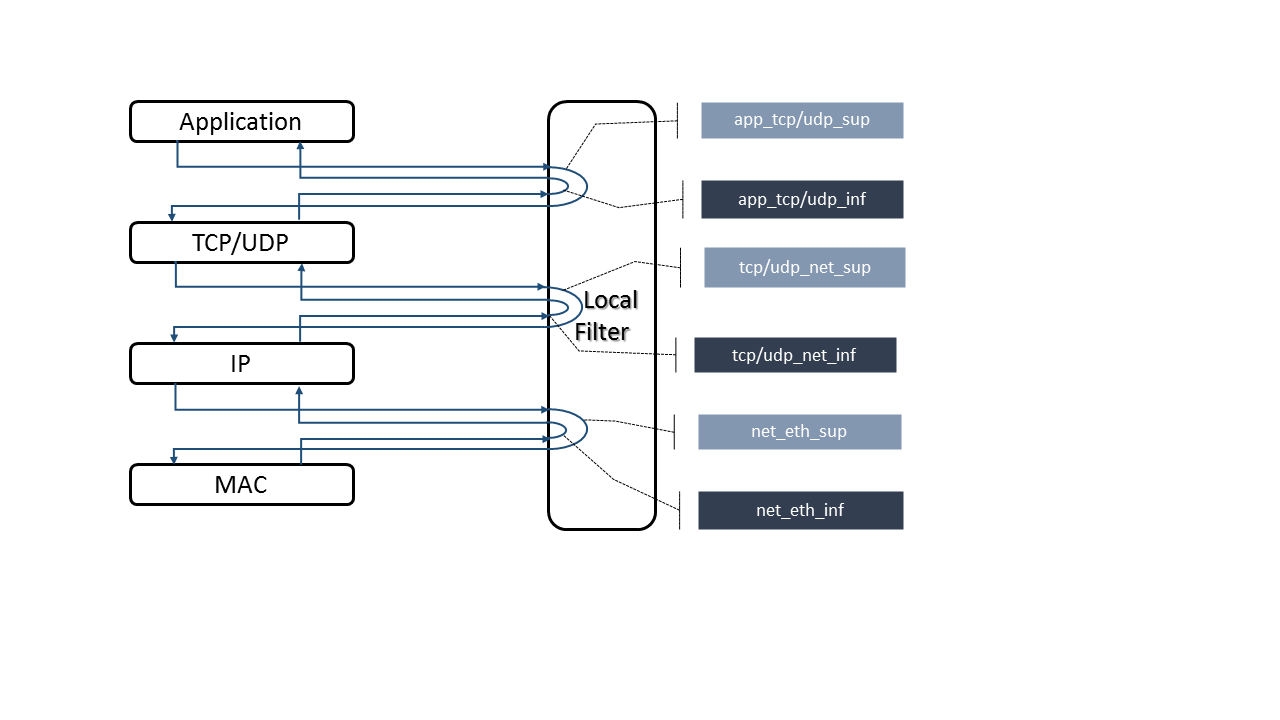
\includegraphics[width=1.5\columnwidth]{LFGates}
\caption{Gates of Local Filter}
\label{img:LFGates}
\end{figure}



% 5-4
\begin{table} [ppp]
\centering
\ttfamily
\footnotesize
\caption{ControlInfo object structure}
\label{tab:from5-to4}
\begin{tabular}{|l|l|l|l|}
\hline
\multicolumn{4}{|c|}{\normalfont\textbf{From layer 5 to layer 4}}	\\
\hline
\multicolumn{1}{|c|}{\normalfont\textbf{ASL type}}	&\multicolumn{1}{c|}{\normalfont\textbf{Packet type}}	&\multicolumn{1}{c|}{\normalfont\textbf{ControlInfo object}}		&\multicolumn{1}{c|}{\normalfont\textbf{fields}}\\
\hline
\multirow{5}{*}{APP.0000}	&\multirow{5}{*}{cPacket}		&\multirow{5}{*}{UDPSendCommand}	&sockId			\\
					&						&								&destAddr	\\
					&						&								&destPort	\\
					&						&								&srcAddr	\\
					&						&								&interfaceId	\\
\hline
\multirow{2}{*}{APP.0100}	&\multirow{2}{*}{cPacket}		&\multirow{2}{*}{TCPSendCommand}	&connId			\\
					&						&								&userId	\\
\hline
\multirow{5}{*}{APP.0201}	&\multirow{5}{*}{TimingReport}	&\multirow{5}{*}{UDPSendCommand}	&sockId			\\
					&						&								&destAddr	\\
					&						&								&destPort	\\
					&						&								&srcAddr	\\
					&						&								&interfaceId	\\
\hline
\multirow{5}{*}{APP.0301}	&\multirow{5}{*}{TimingCommand}	&\multirow{5}{*}{UDPSendCommand}	&sockId			\\
					&							&								&destAddr	\\
					&							&								&destPort	\\
					&							&								&srcAddr	\\
					&							&								&interfaceId	\\
\hline
\end{tabular}
\end{table}

% 4-5
\begin{table} [ppp]
\centering
\ttfamily
\footnotesize
\caption{ControlInfo object structure}
\label{tab:from4-to5}
\begin{tabular}{|l|l|l|l|}
\hline
\multicolumn{4}{|c|}{\normalfont\textbf{From layer 4 to layer 5}}	\\
\hline
\multicolumn{1}{|c|}{\normalfont\textbf{ASL type}}	&\multicolumn{1}{c|}{\normalfont\textbf{Packet type}}	&\multicolumn{1}{c|}{\normalfont\textbf{ControlInfo object}}		&\multicolumn{1}{c|}{\normalfont\textbf{fields}}\\
\hline
\multirow{8}{*}{APP.0000}	&\multirow{8}{*}{cPacket}		&\multirow{8}{*}{UDPDataIndication}		&sockId			\\
					&						&								&srcAddr	\\
					&						&								&destAddr	\\
					&						&								&srcPort	\\
					&						&								&destPort	\\
					&						&								&ttl	\\
					&						&								&interfaceId	\\
					&						&								&typeOfService	\\					
\hline
\multirow{2}{*}{APP.0100}	&\multirow{2}{*}{cPacket}		&\multirow{2}{*}{TCPCommand}	&connId			\\
					&						&								&userId	\\
\hline
\end{tabular}
\end{table}




\iffalse
\begin{table} [ppp]
\centering
\footnotesize
\caption{ControlInfo object structure}
\label{tab:from5-to4}
\ttfamily
\begin{tabular}{|l|l|l|}
\hline
\multicolumn{3}{|c|}{\normalfont\textbf{From layer 5 to layer 4}}	\\
\hline
\multicolumn{1}{|c|}{\normalfont\textbf{ASL type}}	&\multicolumn{1}{c|}{\normalfont\textbf{ControlInfo object}}		&\multicolumn{1}{c|}{\normalfont\textbf{fields}}\\
\hline
\multirow{5}{*}{APP.0000}	&\multirow{5}{*}{UDPSendCommand}	&sockId			\\
					&								&destAddr			\\
					&								&destPort			\\
					&								&srcAddr			\\
					&								&interfaceId		\\
\hline
% removed rows
\iffalse
\multirow{3}{*}{APP.0001}	&\multirow{3}{*}{UDPBindCommand}		&sockId			\\
					&								&localAddr		\\
					&								&localPort			\\
\hline
\multirow{3}{*}{APP.0002}	&\multirow{3}{*}{UDPConnectCommand}	&sockId			\\
					&								&remoteAddr		\\
					&								&remotePort		\\
\hline
APP.0003				&UDPCloseCommand				&sockId			\\
\hline
\fi
%
\multirow{2}{*}{APP.0100}	&\multirow{2}{*}{TCPSendCommand}	&connId			\\
					&								&userId			\\
\hline
% removed rows
\iffalse
\multirow{9}{*}{APP.0101}	&\multirow{9}{*}{TCPOpenCommand}	&connId			\\
					&								&userId			\\
					&								&localAddr		\\
					&								&remoteAddr		\\
					&								&localPort			\\
					&								&remotePort		\\
					&								&fork				\\
					&								&dataTransferMode	\\
					&								&tcpAlgorithmClass	\\
\hline
\fi
\multirow{5}{*}{APP.0201}	&\multirow{5}{*}{TimingReportUDP}	&sockId			\\
					&								&destAddr			\\
					&								&destPort			\\
					&								&srcAddr			\\
					&								&interfaceId		\\
\hline
\multirow{5}{*}{APP.0301}	&\multirow{5}{*}{TimingCommandUDP}	&sockId			\\
					&								&destAddr			\\
					&								&destPort			\\
					&								&srcAddr			\\
					&								&interfaceId		\\
\hline
\end{tabular}
\end{table}


\begin{table} [ppp]
\centering
\ttfamily
\footnotesize
\caption{ControlInfo object structure}
\label{tab:ipv4-control-info}
\begin{tabular}{|l|l|l|}
\hline
\multicolumn{3}{|c|}{\normalfont\textbf{From layer 4 to layer 5}}	\\
\hline
\multicolumn{1}{|c|}{\normalfont\textbf{ASL type}}	&\multicolumn{1}{c|}{\normalfont\textbf{ControlInfo object}}		&\multicolumn{1}{c|}{\normalfont\textbf{fields}}\\
\hline
\multirow{8}{*}{TRA.0000}	&\multirow{8}{*}{UDPDataIndication}		&sockId		\\
					&								&srcAddr		\\
					&								&destAddr		\\
					&								&srcPort		\\
					&								&destPort		\\
					&								&ttl			\\
					&								&interfaceId	\\
					&								&typeOfService	\\
\hline
% removed rows
\iffalse
\multirow{5}{*}{TRA.0001}	&\multirow{5}{*}{UDPErrorIndication}		&sockId		\\
					&								&srcAddr		\\
					&								&destAddr		\\
					&								&srcPort		\\
					&								&destPort		\\
\hline
\multirow{6}{*}{TRA.0010}	&\multirow{6}{*}{TCPConnectInfo}		&connId		\\
					&								&userId		\\
					&								&localAddr	\\
					&								&remoteAddr	\\
					&								&localPort		\\
					&								&remotePort	\\
\hline
\multirow{4}{*}{TRA.0011}	&\multirow{4}{*}{TCPErrorInfo}			&connId		\\
					&								&userId		\\
					&								&errorCode	\\
					&								&messageText	\\
\hline
\fi
%
\multirow{2}{*}{APP.0104}	&\multirow{2}{*}{TCPCommand}		&connId		\\
					&								&userId		\\
\hline
\end{tabular}
\end{table}
\fi





% removed table
\iffalse
\begin{table} [ppp]
\centering
\footnotesize
\caption{ControlInfo object structure}
\label{tab:from5-to4}
\ttfamily
\begin{tabular}{|l|l|l|}
\hline
\multicolumn{3}{|c|}{\normalfont\textbf{From layer 5 to layer 4}}	\\
\hline
\multicolumn{1}{|c|}{\normalfont\textbf{ASL type}}	&\multicolumn{1}{c|}{\normalfont\textbf{ControlInfo object}}		&\multicolumn{1}{c|}{\normalfont\textbf{fields}}\\
\hline
\multirow{5}{*}{APP.0000}	&\multirow{5}{*}{UDPSendCommand}	&sockId			\\
					&								&destAddr			\\
					&								&destPort			\\
					&								&srcAddr			\\
					&								&interfaceId		\\
\hline
\multirow{3}{*}{APP.0001}	&\multirow{3}{*}{UDPBindCommand}		&sockId			\\
					&								&localAddr		\\
					&								&localPort			\\
\hline
\multirow{3}{*}{APP.0002}	&\multirow{3}{*}{UDPConnectCommand}	&sockId			\\
					&								&remoteAddr		\\
					&								&remotePort		\\
\hline
APP.0003				&UDPCloseCommand				&sockId			\\
\hline
\multirow{2}{*}{APP.0100}	&\multirow{2}{*}{TCPSendCommand}	&connId			\\
					&								&userId			\\
\hline
\multirow{9}{*}{APP.0101}	&\multirow{9}{*}{TCPOpenCommand}	&connId			\\
					&								&userId			\\
					&								&localAddr		\\
					&								&remoteAddr		\\
					&								&localPort			\\
					&								&remotePort		\\
					&								&fork				\\
					&								&dataTransferMode	\\
					&								&tcpAlgorithmClass	\\
\hline
\end{tabular}
\end{table}
\fi


% 4-3
\begin{table} [ppp]
\centering
\ttfamily
\footnotesize
\caption{ControlInfo object structure}
\label{tab:from4-to3}
\begin{tabular}{|l|l|l|l|}
\hline
\multicolumn{4}{|c|}{\normalfont\textbf{From layer 4 to layer 3}}	\\
\hline
\multicolumn{1}{|c|}{\normalfont\textbf{ASL type}}	&\multicolumn{1}{c|}{\normalfont\textbf{Packet type}}	&\multicolumn{1}{c|}{\normalfont\textbf{ControlInfo object}}		&\multicolumn{1}{c|}{\normalfont\textbf{fields}}\\
\hline
\multirow{14}{*}{TRA.0000}	&\multirow{14}{*}{UDPPacket}		&\multirow{14}{*}{IPv4ControlInfo}	&destAddr			\\
						&							&							&srcAddr	\\
						&							&							&interfaceId	\\
						&							&							&multicastLoop	\\
						&							&							&protocol	\\
						&							&							&typeOfService		\\
						&							&							&timeToLive	\\
						&							&							&dontFragments	\\
						&							&							&nextHopAddr	\\
						&							&							&moreFragments	\\
						&							&							&macSrc	\\
						&							&							&macDest	\\
						&							&							&diffServCodePoint			\\
						&							&							&explicitCongestionNotification	\\
\hline
\multirow{14}{*}{TRA.0010}	&\multirow{14}{*}{TCPSegment}	&\multirow{14}{*}{IPv4ControlInfo}	&destAddr			\\
						&							&							&srcAddr	\\
						&							&							&interfaceId	\\
						&							&							&multicastLoop	\\
						&							&							&protocol	\\
						&							&							&typeOfService		\\
						&							&							&timeToLive	\\
						&							&							&dontFragments	\\
						&							&							&nextHopAddr	\\
						&							&							&moreFragments	\\
						&							&							&macSrc	\\
						&							&							&macDest	\\
						&							&							&diffServCodePoint			\\
						&							&							&explicitCongestionNotification	\\
\hline
\end{tabular}
\end{table}
%
\begin{table} [ppp]
\centering
\ttfamily
\footnotesize
\caption{ControlInfo object structure}
\label{tab:from3-to4}
\begin{tabular}{|l|l|l|l|}
\hline
\multicolumn{4}{|c|}{\normalfont\textbf{From layer 3 to layer 4}}	\\
\hline
\multicolumn{1}{|c|}{\normalfont\textbf{ASL type}}	&\multicolumn{1}{c|}{\normalfont\textbf{Packet type}}	&\multicolumn{1}{c|}{\normalfont\textbf{ControlInfo object}}		&\multicolumn{1}{c|}{\normalfont\textbf{fields}}\\
\hline
\multirow{14}{*}{TRA.0000}	&\multirow{14}{*}{UDPPacket}		&\multirow{14}{*}{IPv4ControlInfo}	&destAddr			\\
						&							&							&srcAddr	\\
						&							&							&interfaceId	\\
						&							&							&multicastLoop	\\
						&							&							&protocol	\\
						&							&							&typeOfService		\\
						&							&							&timeToLive	\\
						&							&							&dontFragments	\\
						&							&							&nextHopAddr	\\
						&							&							&moreFragments	\\
						&							&							&macSrc	\\
						&							&							&macDest	\\
						&							&							&diffServCodePoint			\\
						&							&							&explicitCongestionNotification	\\
\hline
\multirow{14}{*}{TRA.0010}	&\multirow{14}{*}{TCPSegment}	&\multirow{14}{*}{IPv4ControlInfo}	&destAddr			\\
						&							&							&srcAddr	\\
						&							&							&interfaceId	\\
						&							&							&multicastLoop	\\
						&							&							&protocol	\\
						&							&							&typeOfService		\\
						&							&							&timeToLive	\\
						&							&							&dontFragments	\\
						&							&							&nextHopAddr	\\
						&							&							&moreFragments	\\
						&							&							&macSrc	\\
						&							&							&macDest	\\
						&							&							&diffServCodePoint			\\
						&							&							&explicitCongestionNotification	\\
\hline
\end{tabular}
\end{table}


% 3 - 2
\begin{table} [ppp]
\centering
\ttfamily
\footnotesize
\caption{ControlInfo object structure}
\label{tab:from3-to2}
\begin{tabular}{|l|l|l|l|}
\hline
\multicolumn{4}{|c|}{\normalfont\textbf{From layer 3 to layer 2}}	\\
\hline
\multicolumn{1}{|c|}{\normalfont\textbf{ASL type}}	&\multicolumn{1}{c|}{\normalfont\textbf{Packet type}}	&\multicolumn{1}{c|}{\normalfont\textbf{ControlInfo object}}		&\multicolumn{1}{c|}{\normalfont\textbf{fields}}\\
\hline
\multirow{1}{*}{NET.0000}&\multirow{1}{*}{IPv4Datagram}		&none	&none	\\
\hline
\multirow{8}{*}{NET.0010}&\multirow{8}{*}{IPv4Datagram}		&\multirow{8}{*}{Ieee802Ctrl}	&src			\\
												&						&									&dest		\\
												&					&									&etherType	\\
												&					&									&interfaceId	\\
												&					&									&switchPort	\\
												&					&									&ssap		\\
												&					&									&dsap		\\
												&					&									&pauseUnits	\\
\hline
\end{tabular}
\end{table}
%
\begin{table} [ppp]
\centering
\ttfamily
\footnotesize
\caption{ControlInfo object structure}
\label{tab:from2-to3}
\begin{tabular}{|l|l|l|l|}
\hline
\multicolumn{4}{|c|}{\normalfont\textbf{From layer 2 to layer 3}}	\\
\hline
\multicolumn{1}{|c|}{\normalfont\textbf{ASL type}}	&\multicolumn{1}{c|}{\normalfont\textbf{Packet type}}	&\multicolumn{1}{c|}{\normalfont\textbf{ControlInfo object}}		&\multicolumn{1}{c|}{\normalfont\textbf{fields}}\\
\hline
\multirow{1}{*}{NET.0000}&\multirow{1}{*}{IPv4Datagram}		&-						&-	\\
\hline
\multirow{8}{*}{NET.0010}&\multirow{8}{*}{IPv4Datagram}		&\multirow{8}{*}{Ieee802Ctrl}	&src			\\
												&						&									&dest		\\
												&						&									&etherType	\\
												&						&									&interfaceId	\\
												&						&									&switchPort	\\
												&						&									&ssap		\\
												&						&									&dsap		\\
												&						&									&pauseUnits	\\
\hline
\end{tabular}
\end{table}


% 2 - 1
\begin{table} [ppp]
\centering
\ttfamily
\footnotesize
\caption{ControlInfo object structure}
\label{tab:from2-to1}
\begin{tabular}{|l|l|l|l|}
\hline
\multicolumn{4}{|c|}{\normalfont\textbf{From layer 2 to layer 1}}	\\
\hline
\multicolumn{1}{|c|}{\normalfont\textbf{ASL type}}	&\multicolumn{1}{c|}{\normalfont\textbf{Packet type}}		&\multicolumn{1}{c|}{\normalfont\textbf{ControlInfo object}}		&\multicolumn{1}{c|}{\normalfont\textbf{fields}}\\
\hline
\multirow{1}{*}{MAC.0000}&\multirow{1}{*}{PPPFrame}		&-	&-	\\
\hline
\multirow{1}{*}{MAC.0010}&\multirow{1}{*}{EthernetFrame}	&-	&-	\\
\hline
\multirow{1}{*}{MAC.0020}&\multirow{1}{*}{IdealAirFrame}		&-	&-	\\
\hline
\multirow{1}{*}{MAC.0030}&\multirow{1}{*}{AirFrame}		&-	&-	\\
\hline
\end{tabular}
\end{table}
%
\begin{table}[ppp]
\centering
\ttfamily
\footnotesize
\caption{ControlInfo object structure}
\label{tab:from1-to2}
\begin{tabular}{|l|l|l|l|}
\hline
\multicolumn{4}{|c|}{\normalfont\textbf{From layer 1 to layer 2}}	\\
\hline
\multicolumn{1}{|c|}{\normalfont\textbf{ASL type}}	&\multicolumn{1}{c|}{\normalfont\textbf{Packet type}}		&\multicolumn{1}{c|}{\normalfont\textbf{ControlInfo object}}		&\multicolumn{1}{c|}{\normalfont\textbf{fields}}\\
\hline
\multirow{1}{*}{MAC.0000}&\multirow{1}{*}{PPPFrame}		&-	&-	\\
\hline
\multirow{1}{*}{MAC.0010}&\multirow{1}{*}{EthernetFrame}	&-	&-	\\
\hline
\multirow{1}{*}{MAC.0020}&\multirow{1}{*}{IdealAirFrame}		&-	&-	\\
\hline
\multirow{1}{*}{MAC.0030}&\multirow{1}{*}{AirFrame}		&-	&-	\\
\hline
\end{tabular}
\end{table}









\iffalse
\begin{landscape}
%\begin{sidewisetable}
\begin{table} [ppp]
\centering
\footnotesize
\caption{ASL type and and relative protocol commands (i.e. ControlInfo object classes)}
\label{tab:control-info}
\ttfamily
\begin{tabular}{|c|l|l|l|l|l|l|l|l|}
\hline
\diagbox{\normalfont\textbf{from}}{\normalfont\textbf{to}}	& \multicolumn{2}{c|}{\normalfont\textbf{layer 5}}	& \multicolumn{2}{c|}{\normalfont\textbf{layer 4}}		& \multicolumn{2}{c|}{\normalfont\textbf{layer 3}}		& \multicolumn{2}{c|}{\normalfont\textbf{layer 2}} \\
\hline
\multirow{4}{*}{\normalfont\textbf{layer 5}}		&			& 					&APP.0000	&UDPSendCommand	&	& 	&	& 	\\
%									&			& 					&APP.0001	&UDPBindCommand	&	& 	&	& 	\\
%									&			& 					&APP.0002	&UDPConnectCommand	&	& 	&	& 	\\
%									&			& 					&APP.0003	&UDPCloseCommand	&	& 	&	& 	\\
									&			& 					&APP.0100	&TCPSendCommand	&	& 	&	& 	\\
%									&			& 					&APP.0101	&TCPOpenCommand	&	& 	&	& 	\\
									&			& 					&APP.0201	&TimingReportUDP		&	& 	&	& 	\\
									&			& 					&APP.0301	&TimingComandUDP	&	& 	&	& 	\\
									
\hline
\multirow{2}{*}{\normalfont\textbf{layer 4}}		&APP.0004	&UDPDataIndication 	&			& 					&TRA.0000	&UDPoverIPv4	&	& 	\\
								%	&APP.0005	&UDPErrorIndication 	&			& 					&TRA.0001	&TCPoverIPv4 	&	& 	\\
								%	&APP.0102	&TCPConnectInfo		&			&					&			& 	&	& 	\\
								%	&APP.0103	&TCPErrorInfo			&			&					&			& 	&	& 	\\
									&APP.0104	&TCPCommand		&			&					&TRA.0001	&TCPoverIPv4 	&	& 	\\
\hline
\multirow{2}{*}{\normalfont\textbf{layer 3}}		&			& 					&TRA.0000	&UDPoverIPv4			&	& 	&NET.0000	&IPv4Datagram 		\\
									&			& 					&TRA.0001	&TCPoverIPv4			&	& 	&NET.0001	&IPv4Datagram802Ctrl	\\
\hline
\multirow{2}{*}{\normalfont\textbf{layer2}}		&			&				 	&			& 					&NET.0000	&IPv4Datagram 		&	& 	\\
									&			& 					&			&					&NET.0000	&IPv4Datagram802Ctrl 	&	& 	\\
\hline

\multicolumn{1}{l|}{}    			& \normalfont\textbf{ASL type}   & \normalfont\textbf{ControlInfo object}  
								& \normalfont\textbf{ASL type}   & \normalfont\textbf{ControlInfo object}
									& \normalfont\textbf{ASL type}   & \normalfont\textbf{ControlInfo object}
										& \normalfont\textbf{ASL type}   & \normalfont\textbf{ControlInfo object}\\
\cline{2-9}
\end{tabular}
%\end{sidewaystable}
\end{table}
\end{landscape}
\fi